\documentclass{beamer}
\usetheme{CambridgeUS}

%\usepackage{listings}
%\lstset{language=bash}

\usepackage[english,francais]{babel}
\usepackage[utf8]{inputenc}
%\usepackage[latin1]{inputenc}
\usepackage{verbatim}
%\usepackage{isolatin1}

\title{OAR}
\subtitle{Un gestionnaire de tâches et de ressource pour grandes grappes de calcul}
\author{Olivier~Richard \and Bruno~Bzeznik \and Romain~Cavagna \and Joseph~Emeras}
\institute{ LIG / CIMENT / ALADDIN-G5K }
\date{JRES - 3 decembre 2009}


\begin{document}

\frame{
	\titlepage

    \begin{center}

        \includegraphics[height=7ex]{img/oar_logo.png} \\

        \includegraphics[height=6ex]{img/LIG_coul.jpg}
        \hspace{2ex}
        \includegraphics[height=3ex]{img/cnrs.jpg}
        \hspace{1ex}
        \includegraphics[height=3ex]{img/logo_inpg.jpg}
        \hspace{1ex}
        \includegraphics[height=3ex]{img/inria.jpg} \\
        \hspace{1ex}
        \includegraphics[height=3ex]{img/logo_ujf.jpg}
        \hspace{1ex}
        \includegraphics[height=5ex]{img/logo_upmf.jpg}
        \hspace{1ex}
        \includegraphics[height=2ex]{img/ciment-logo2.jpg}
        \hspace{1ex}
        \includegraphics[height=5ex]{img/Logo_Aladdin.png}
    \end{center}
	}

\frame{
  \frametitle{Sommaire}
  	\tableofcontents
}

\section{Généralités}

\frame{
 \frametitle{Les Gestionnaires de tâches et de ressources}
	
    \begin{itemize}
	\item Aussi appelés {\em Batch Scheduler}
        \item Contexte: {\bf High Performance Computing} (Supercalculateurs, Grappes de calcul, Clusters)
	\item Existent en très grand-nombre: {\bf Condor }, {\bf Sun Grid Engine (SGE)}, {\bf MAUI/Torque}, {\bf Slurm}, {\bf OAR}, {\bf Catalina}, {\em LSF }, {\bf Lava}, {\em PBS Pro}, {\em Moab}, Loadleveler, CCS...
        \item \url{http://en.wikipedia.org/wiki/Job_scheduler}
  \end{itemize}

}

\begin{frame}
	\frametitle{Principe général}

	Dans leur version simple, les gestionnaires de tâches et de ressources sont séparés en 2 couches (parfois une 3éme Workload Managment) :
	
	\begin{center}
			\includegraphics[width=6cm]{img/task_resources.png}
	\end{center}

\end{frame}

\begin{frame}
	\frametitle{Organisation générale}

	\begin{itemize}
		\item Un serveur central
		\item Des programmes clients (en ligne de commandes) pour l'interaction avec les utilisateurs
		\item Une grande latitude dans le paramétrage
	\end{itemize}

	\begin{center}
		\includegraphics[height=4cm]{Batch_organization.pdf}
	\end{center}

\end{frame}

\section{Fonctionnaliés communes}

\begin{frame}
\frametitle{Fonctionnalités (1/2)}
	{\bf liste non-exhaustive}
		\begin{itemize}
		\item Tâche ({\em soumission}) Interactive (shell) / Batch
		\item Tâche séquentielle et parallèle
		\item Walltime (temps limite). ({\bf important pour l'ordonnancement)}
		\item Accès exclusif / non-exclusif aux ressources 
		\item Appariement de ressources
		\item Scripts Epilogue/Prologue (exécuter avant/après les tâches)
		\item Suivi ({\em monitoring}) des tâches (consommation des ressources)
		\item Dépendance entre tâches ({\em workflow})
		\item Logging et accounting
		\item Suspension/reprise des tâches 
	\end{itemize}
\end{frame}

\begin{frame}
\frametitle{Fonctionnalités (2/2)}
	{\bf liste non-exhaustive}
		\begin{itemize}
    \item Tableaux de tâches
		\item First-Fit (Conservative Backfilling,)
		\item Fairsharing
    \item ... 
		
	\end{itemize}
\end{frame}


\section{Objectifs et fonctionnalités de OAR}


\begin{frame}
	\frametitle{Objectifs} \hypertarget{objectifs}{}

	OAR: Un gestionnaire de tâches et de ressources {\bf polyvalent} et {\bf {\em personnalisable}}.

	\begin{itemize}
		\item Suivre l'évolution technologique (machine et infrastructure de plus en plus complexe)
		\item Contexte initial: CIMENT \hyperlink{ciment-appendix}{ \beamergotobutton{...}}  et Grid5000 \hyperlink{g5k-appendix}{ \beamergotobutton{...}}
                \item Adaptation aux différents contextes (cluster, cluster-on-demand, cluster virtuel, multi-cluster, grille légère, plate-forme pour l'expérimentation à la Grid'5000, {\em grand cluster}, besoin spécifique). 
	\end{itemize}

\begin{center}
        \hspace{1ex}
        \includegraphics[height=2ex]{img/ciment-logo2.jpg}
        \hspace{1ex}
        \includegraphics[height=7ex]{img/Logo_Aladdin.png}
\end{center}

%\begin{alertblock}{Sous-estimation}
%   Regle des 80/20 : les 20\% des fonctionnalités {\bf ne sont pas les mêmes pour tous !!!}  
%\end{alertblock}

\end{frame}

\frame{
\frametitle{Eco-système}
  \begin{center}
    \includegraphics[width=11cm]{global_picture.png}
  \end{center}
}

\begin{frame}
\frametitle{Fonctionnalités et spécifités de OAR}
	{\bf liste non-exhaustive}
		\begin{itemize}
    \item Fonctionnalités classiques +
    \item Advance Reservation
		\item {\bf Expression des hiérarchies dans les requêtes }
		\item {\bf Support de ressources de type différent (ex licence, capacité de stockage, capacité réseaux...)  }
		\item {\bf Tâche container} ({\em récursivité, soumettre dans une tâche})
		\item {\bf Tâche besteffort} (tâche à priorité nulle, très utilisé par {\em CiGri}) 
		\item {\bf Type multiple de tâches} (besteffort, deploy, timesharing, idempotent, power, cosystem ...) (personnalisable)
    \item {\bf Tâches moldables}
    \item {\bf Economie d'énergie}
		%\item First-Fit (Conservative Backfilling,)
		%\item Fairsharing 
		
	\end{itemize}
\end{frame}




\section{Principes et architecture}
%% Principe
\frame{
  \frametitle{OAR: principes de conception}
Utilisation de composants logiciels de haut niveau
   \begin{itemize}
    \item {\bf Base de donnée relationnelle} (MySql/PostgreSQL) au coeur du système pour stocker et échanger
      %\begin{itemize}
      %  \item Information sur les ressources et les tâches 
      %  \item L'état interne du système
      % \end{itemize}
    \item {\bf Language(s) de script} (Perl, Ruby) pour le moteur d'exécution et les modules (interchangeables)
    %\begin{itemize}
    % \item Bien adapté pour les parties systèmes
    % \item Structures de haut niveau (listes, tables associatives, tris...)
    % \item Cycles de développement court
    % \end{itemize}
    \item {\bf Autres composants}: SSH, CPUSETS, Taktuk
    %\begin{itemize}
    %  \item \textbf{SSH, CPUSET} (confinement, nettoyage)
    %  \item \textbf{Taktuk} lanceur parallèle adaptatif et polyvalent
    %\end{itemize}
  \end{itemize}
	\begin{center}
		\includegraphics[height=3cm]{OAR_organization.pdf}
	\end{center}

}

%\frame{
%	\frametitle{OAR : organisation générale}
%
%	La base de donnée a un rôle central
%
%	\begin{itemize}
%		\item {\bf l'état interne simplement accessible}
%		\item le moteur est composé de {\bf petit modules Perl}
%		\item chaque module (= un script) peut-être facilement remplacé
%	\end{itemize}
%
%	\begin{center}
%		\includegraphics[height=3cm]{OAR_organization.pdf}
%	\end{center}
%}

\begin{frame}
\frametitle{Cycle d'un job}
	\begin{center}
		\includegraphics[width=10cm]{cycle_job.png}
	\end{center}
\end{frame}


\frame{
  \frametitle{Règles d'admissions}
  \begin{alertblock}{Un point de paramétrage important}
    \begin{itemize}
      \item Grandes possibilités de {\em personnalisation} pour l'administrateur
      \item {\bf Cadrage} des requêtes
      \item fixe des valeurs par défaut: walltime, queue, nombre de ressources demandées, 
      \item contrôle d'accès (utilisateur, groupe, plage horaire...)
    \end{itemize}
  \end{alertblock}
}


\frame{
	\frametitle{Diagramme d'état d'une tâche}
	%Exemple du système OAR (version 1.6)
	\includegraphics[width=\textwidth]{JobStates.pdf}
}

\begin{frame}
	\frametitle{Exemples de soumission: OAR}
	
Soumission pour tâche interactive: \footnote{{\bf Note:} Chacune des commandes de soumission renseigne un numéro de tâche.}

		\begin{itemize}
			\item	{\bf oarsub -l nodes=4 -i}
		\end{itemize}

	Soumission en {\em batch} (avec {\em walltime} et choix de queue):
		\begin{itemize}
			\item	{\bf oarsub -q default -l walltime=2:00,nodes=10 /home/toto/script}
		\end{itemize}

	Soumission d'une réservation:
		\begin{itemize}
			\item	{\bf oarsub -r "2008-04-27 11:00" -l nodes=12}
		\end{itemize}

	Connexion à une réservation (utilise le numéro de tâche):
		\begin{itemize}
			\item	{\bf oarsub -C 154}
		\end{itemize}


\end{frame}

\section{Ordonnancement}

% FIFO, BACKFILLING, FAIRSHARING, Advance reservartion, PRIORITE, BEST-EFFORT récursivité

\begin{frame}
	\frametitle{Ordonnancement}
	
	L'ordonnancement est l'étape \footnote{{\bf Note:} l'ordonnancement est recalculé à chaque changement d'état (majeur) d'une tâche.}
où le système choisi les {\bf ressources à attribuées} aux tâches et {\bf les dates de lancement}.
\\[0.4cm]
	L'ordonnancement est défini suivant une {\bf politique} qui se traduit par l'utilisation {\bf d'algorithmes d'ordonnancement}.
\\[0.4cm]
	{\bf De plus} de nombreux {\bf critères et paramètres} sont utilisés pour guider et cadrer les allocations et les priorités.
 

\end{frame}

\frame{
	\frametitle{Organisation de l'ordonnancement}
	Gestion des tâches par file (queues)
	\begin{itemize}
		\item chaque file a une priorité
		\item chaque file a sa propre politique d'ordonnancement
	\end{itemize}
%equivalent to scheduling jobs with priorities but easier to administrate
\includegraphics[width=\textwidth]{schedule_eng.pdf}
}

\frame{
	\frametitle{Appariement de ressource / ressource matching}

  \begin{block}{Une étape préliminaire à l'ordonnancement}
    \begin{itemize}
      \item {\bf Filtrage} de resources
      \item {\bf Classement} de ressources 
      \item Permet de spécifier des besoins particuliers
      \item mémoire, architecture, machine particulières, OS, niveau de charge...    
    \end{itemize}
  \end{block}

%  Condor / ClassAds : Syntaxe, Attributs, Opérateurs, Classement (Ranking)
}




\begin{frame}
	\frametitle{Politiques d'ordonnancement}
		\begin{itemize}
		\item FIFO (First-In First-Out)
		\item First-Fit (Backfilling)
		\item FairSharing
		\item Timesharing
		\item Advance reservation
		\item Récursivité
	\end{itemize}

\end{frame}

\begin{frame}
	\frametitle{FIFO: Fisrt-In First-Out}
	\begin{center}
		\includegraphics[width=7cm]{fifo.png}
	\end{center}

\end{frame}

\begin{frame}
	\frametitle{ First-Fit (Backfilling)}
	Remplissage des trous si l'ordre des tâches soumises antérieurement n'est pas modifié
	\begin{center}
			\includegraphics[width=6cm]{fifo.png}
		\includegraphics[width=6cm]{cbf.png}
	\end{center}

\end{frame}

\begin{frame}
	\frametitle{FairSharing (partage équitable)}
	L'ordre est calculé suivant ce qui a été consommé (on favorise les utilisateurs peu gourmands). Définition d'une fenêtre et paramètres de pondération.
	\begin{center}
		\includegraphics[width=6cm]{fifo.png}
		\includegraphics[width=6cm]{fairsharing.png}
	\end{center}
\end{frame}

\begin{frame}
	\frametitle{Réservation ({\em Advance Reservation})}

		\begin{itemize}
		\item {\bf Très pratique} pour démo, planification, tâche multi-site ou de type grille...
		\item {\bf Mais}
			\begin{itemize}
				\item Contraignant pour l'ordonnanceur (attention au niveau d'utilisation)
				\item Les ressources sont rarement utilisée sur toute la durée (gaspillage)
			\end{itemize}
		\end{itemize}

	\begin{center}
		\includegraphics[width=6cm]{resa.png}
	\end{center}
	{\bf oarsub -r "2008-04-27 11:00" -l nodes=12}

\end{frame}

\begin{frame}
  \frametitle{TimeSharing} 
  \begin{center}
			\includegraphics[width=7cm]{timesharing.png}
	\end{center}
\end{frame}

\begin{frame}
  \frametitle{Récursivité}
  Faire de l'ordonnancement dans une allocation/réservation. Intéressant pour formation, démo, partage de ressource plus flexible  par groupe d'utilisateurs / projet. {\bf Tâche de type container.} 
  \begin{center}
			\includegraphics[width=7cm]{recursivity.png}
	\end{center}

\end{frame}

\section{Contraintes Topologiques}

\frame{
\frametitle{Contraintes Topologiques} \hypertarget{topo}{}
  \begin{block}{Evolution du matériel}
    \begin{itemize}
      \item switch/noeud/cpu/core: \alert{Architecture Hierarchique}
      \item machine NUMA / machine BlueGene: \alert{Architecture en grille 2D, 3D ou hybride} \hyperlink{topo-appendix}{ \beamergotobutton{...}}
    \end{itemize}
  \end{block}
  \begin{center}
  \includegraphics[width=9cm]{img/cluster_hierar.png}
  \end{center}
}

\frame{
\frametitle{Contraintes Topologiques hiérarchiques}
Problème avec les applications parallèles sensible au débit communication.
\begin{center}
  \includegraphics[width=9cm]{img/cluster_hierar_app.png}
  \end{center}
}

\frame{
\frametitle{Contraintes Topologiques hiérarchiques}

\begin{itemize}
 \item Notion de hiérarchie dans les requetes:
  \\
  {\bf oarsub -l switch=1/nodes=2/cpu=2/core=2 appli-parallèle}
   \\        = 1x2x2x2 = 8 coeurs
 \item Gestion des cpusets linux (attention à l'affinité même au sein d'un cpuset)
\end{itemize}
}


%\frame{
%  \frametitle{Application parallèle et affinité processeur}
% 
%  {\bf Note:} CPUSET ensemble de coeurs et/ou CPU sur un noeud.
%
%\begin{block}{}
%
%	  \begin{enumerate}
%  	  \item L'attribution CPUSET/core pour application parallèle peut ne pas suffire
%      \item Problème de l'ordonnanceur de l'OS (ici souvent Linux), le processus change de coeur à l'intérieur des CPUSET 
% 		  \item Il faut utilisé les capacités de verrouillage sur coeur ({\em Processor Affinity})
%	  \end{enumerate}
%
%\end{block}
% 
%}

%%% TODO
%%% Energie
%%% Tolérance aux pannes
%%% API
%%% GUI

\section{Energie}

\begin{frame}
  \frametitle{Gestion de l'énergie} \hypertarget{energy}{}
  \begin{itemize}
    \item {\bf Arrêt des machines inutilisées (réveil aux besoins)}
    \item Priorité heures creuses/pleines par paramétrage
		\item Développées lors du {\em Google Summer Of Code 2008} (Gsoc'08)
    \begin{itemize}
       \item Un nouveau type de job paramétrique:  {\bf powersaving} + options (cpufreq, arrêt sélectif de périphérique disque, video ..., politique spécifique)
       \item Ex Job BestEffort $\rightarrow$ fréquence CPU la plus faible.
    \end{itemize}
  \end{itemize}
  \begin{center}
    \includegraphics[width=3cm]{img/energy50.png}
    \includegraphics[width=3cm]{img/energy90.png}
    \\\hyperlink{energy-appendix}{\beamergotobutton{...}}
  \end{center}
\end{frame}


\section{Interfaces}

\frame{
  \frametitle{OAR: Monika}
  \begin{center}
  \includegraphics[width=7cm]{img/monika.png}
  \end{center}
}


\frame{
  \frametitle{OAR: Diagramme de Gantt}
  \includegraphics[width=\textwidth]{gantt_ita.png}
}


\begin{frame}
  \frametitle{API REST}

  \begin{block}{}
    \begin{itemize}
      \item REST = protocole HTTP PUT/GET/POST/DELETE sur des ressources 
      \item {\bf Interface simple et puissante !}
      \item Pas la lourdeur des Web Services à la Soap.  
    \end{itemize}
  \end{block}

  \begin{block}{}
    \begin{itemize}
      \item {\bf  \url{http://mydomain.org/oarapi/resources.json} }
      \item  Donne la liste de toutes les ressources de la grappe au format json 
    \end{itemize}
  \end{block}

%\begin{verbatim}
%# Get the list of resources
%wget -O - http://mydomain.org/oarapi/resources.yaml?structure=simple
%\end{verbatim}

\end{frame}

\frame{
  \frametitle{Exemple d'utilisation de l'interface REST}
  \begin{center}
    \includegraphics[width=6cm]{img/chandler2.png}
  \end{center}
  {\em Chandler}: en 80 lignes de code, affichage du status des noeuds et des coeurs en mode console.
}


\section{Perspectives et conclusion}

\frame{
  \frametitle{Equipe }
  \begin{block}{Equipe}
  \begin{itemize}
    \item {\bf 1 ingénieur senior (\%50) + 2 ingénieurs CDD + 1 doctorant}
    \item {\bf 1 MdC (direction, codage) + 3 MdC (consultants / codage ponctuel)}
    \item Contributeurs (dont l'ancien ingénieur développeur principal)
    \item 5 stagiaires Gsoc (Google Summer of Code 08 et 09) 
    \item Une 10zaine de personnes qui ont contribués 
  \end{itemize}
 \end{block}
}

\frame{
  \frametitle{Références/support}

  \begin{block}{Réferences}
  \begin{itemize}
    \item Entre 7000 et 15000 coeurs, autour de 30 clusters
    \item Mesocentre CIMENT, Grid'5000, BRGM, Footways, Usharesoft, Université/Labo (France, Chine, Brésil,Luxembourg, US, Slovakie...)
  \end{itemize}
 \end{block}

  \begin{block}{Support}
  \begin{itemize}
    \item OAR Licence GPL
    \item Mailing List, Gestionnaire de Bug
    \item Aide à l'installation (nous ou partenaire ex: BULL/Serviware)
    \item Support Pro (cas par cas)
  \end{itemize}
 \end{block}
}

\frame{
  \frametitle{Perspectives}
  \begin{block}{}
  \begin{itemize}
    \item {\bf Interfacage à gLite} (serveur blahp ?)
    \item {\bf Ordonnanceur (nouvelle version)}
    \item Interface web intégrée
    \item Actuellement de 1000 à 10000 (ressources: noeuds, cpus, coeurs...)
    \item 100K ressources, numa massivement multi-coeur  ?
    \item détection des inéfficacités ?
    \item Environnement de test/ de re-exécution (vision globale ordonnancement et système de fichier)
    \item Cluster virtuel / couplage Boinc
    \item Partenariats BULL, CEA
  \end{itemize}
 \end{block}



}

\frame{
  \frametitle{Conclusion}

 \begin{block}{}
  \begin{itemize}
    \item {\bf Polyvalent et personnalisable}
    \item Niveau de fonctionnalité comparable à la concurrence
    \item Très bonne stabilité
    \item Version stable:  {\bf {\em 2.4.1 (Thriller)}} (.tgz, .deb, .rpm)
    \item Domaine encore en évolution 
  \end{itemize}
 \end{block}
 \begin{center}
    \hspace{-1.5cm}
    \includegraphics[height=9ex]{img/oar_logo.png}
   \end{center} 


}

\frame{
  \begin{center}
		{\huge Des questions ?}
	\end{center}

  \begin{center}
    \hspace{-1.5cm}
    \includegraphics[height=4cm]{img/oar_logo.png}
   \end{center} 

  \begin{center}
    \vspace{-0.5cm}
    {\bf http://oar.imag.fr/}
  \end{center}
}


\begin{frame}
\frametitle{Liens}
\begin{thebibliography}{Resource Management System}

	\bibitem{Condor}
	Condor 
	\newblock {\em http://www.cs.wisc.edu/condor/}

  \bibitem{SGE}
	Sun Grid Engine (SGE) 
	\newblock {\em http://gridengine.sunsource.net}

	\bibitem{TORQUE}
	TORQUE/MAUI
	\newblock {\em http://www.clusterresources.com/}

  \bibitem{SLURM}
	SLURM
	\newblock {\em www.llnl.gov/linux/slurm/}

	\bibitem{LSF}
	LSF
	\newblock {\em http://www.platform.com}

	\bibitem{OAR}
	OAR 
	\newblock {\em http://oar.imag.fr}



\end{thebibliography}
\end{frame}


\section{Annexes}

\frame{
\frametitle{OAR: Historique}
%%% TODO rajoute image icluster
\begin{itemize}
  \item Début 2003: Une machine dans le Top500 (225 noeuds), OpenPBS(Torque) est instable et difficile à faire évoluer 
  \item PBSpro se comporte mieux (passage à l'échelle imparfait)
\end{itemize}

	\begin{center}
  	\includegraphics[width=6cm]{img/icluster1.jpg}
  \end{center}
}

\frame{
\frametitle{Contraintes Topologiques: grille/tore 2D} \hypertarget{topo-appendix}{}
\begin{center}
  \includegraphics[width=9cm]{img/grille_2D_renum.png}
\end{center}
}

\frame{
\frametitle{Contraintes Topologiques: grille/tore 3D}
\begin{itemize}
  \item Courbe de Hilbert (Slurm / topology)
  \item Wikipedia / $Hilbert\_curve$ 
\end{itemize}
\begin{center}
  \includegraphics[width=5cm]{img/Hilbert3d-step3.png}
\end{center}
\hyperlink{topo}{\beamerreturnbutton{Back.}}
}

\frame{
\frametitle{Interfaces:}

\begin{block}{}
  \begin{itemize}
    \item Interface commande en ligne (CLI)
    \item Application exemple DRMAA (v1, v2)
    \item Grille : Globus GT2, GT4/ OGSA-BESS, JSDL, G-Lite - BLAHp, SAGA
    \item Beaucoup d'interface, souvent limitatives ?
  \end{itemize}
 \end{block}

	\begin{center}
			\includegraphics[width=9cm]{img/drmaastack.png}
	\end{center}

  {\bf OAR}: DRMAA (85\%), Glite ({\bf commandée}), REST

}

\frame{
\frametitle{Le mesocentre de calcul CIMENT} \hypertarget{ciment-appendix}{}
  \begin{itemize}
    \item Mesocentre de calcul intensif de l'Université Joseph Fourier (Grenoble)
    \item Une douzaine de calculcateurs hétérogènes, plus de 2000 cores autjourd'hui
    \item Particularité: mutualisation autour d'une grille légère (CiGri)
    \item Forte collaborations production/recherche
  \end{itemize}
\hyperlink{objectifs}{\beamerreturnbutton{Back.}}
}

\frame{
\frametitle{Grid 5000} \hypertarget{g5k-appendix}{}
  \begin{itemize}
    \item Grille pour l'expérimentation informatique
    \item 9 sites en France + 2 sites à l'étranger
    \item Interconnexion gigabit dédiée Renater
    \item Plus de 5000 cores aujourd'hui
  \end{itemize}
\hyperlink{objectifs}{\beamerreturnbutton{Back.}}
}

\frame{ \hypertarget{energy-appendix}{}
	\begin{center}
    \includegraphics[width=9cm]{img/energy50.png}
  \end{center}
}

\frame{
  \begin{center}
    \includegraphics[width=8cm]{img/energy90.png}
  \end{center}
\hyperlink{energy}{\beamerreturnbutton{Back.}}
}

\end{document}

